% scram1.tex
\section{Katsu's scramjet combustor and nozzle}
\label{scram1-sec}
%
The core of Katsuyoshi Tanimizu's scramjet model is shown in 
Figure\,\ref{scram1-core-model-fig}.
It was designed in 1994 by Prof. Ray Stalker and consists of 6 scramjet 
ducts distributed around a centrebody.

\begin{figure}[htbp]
\begin{center}
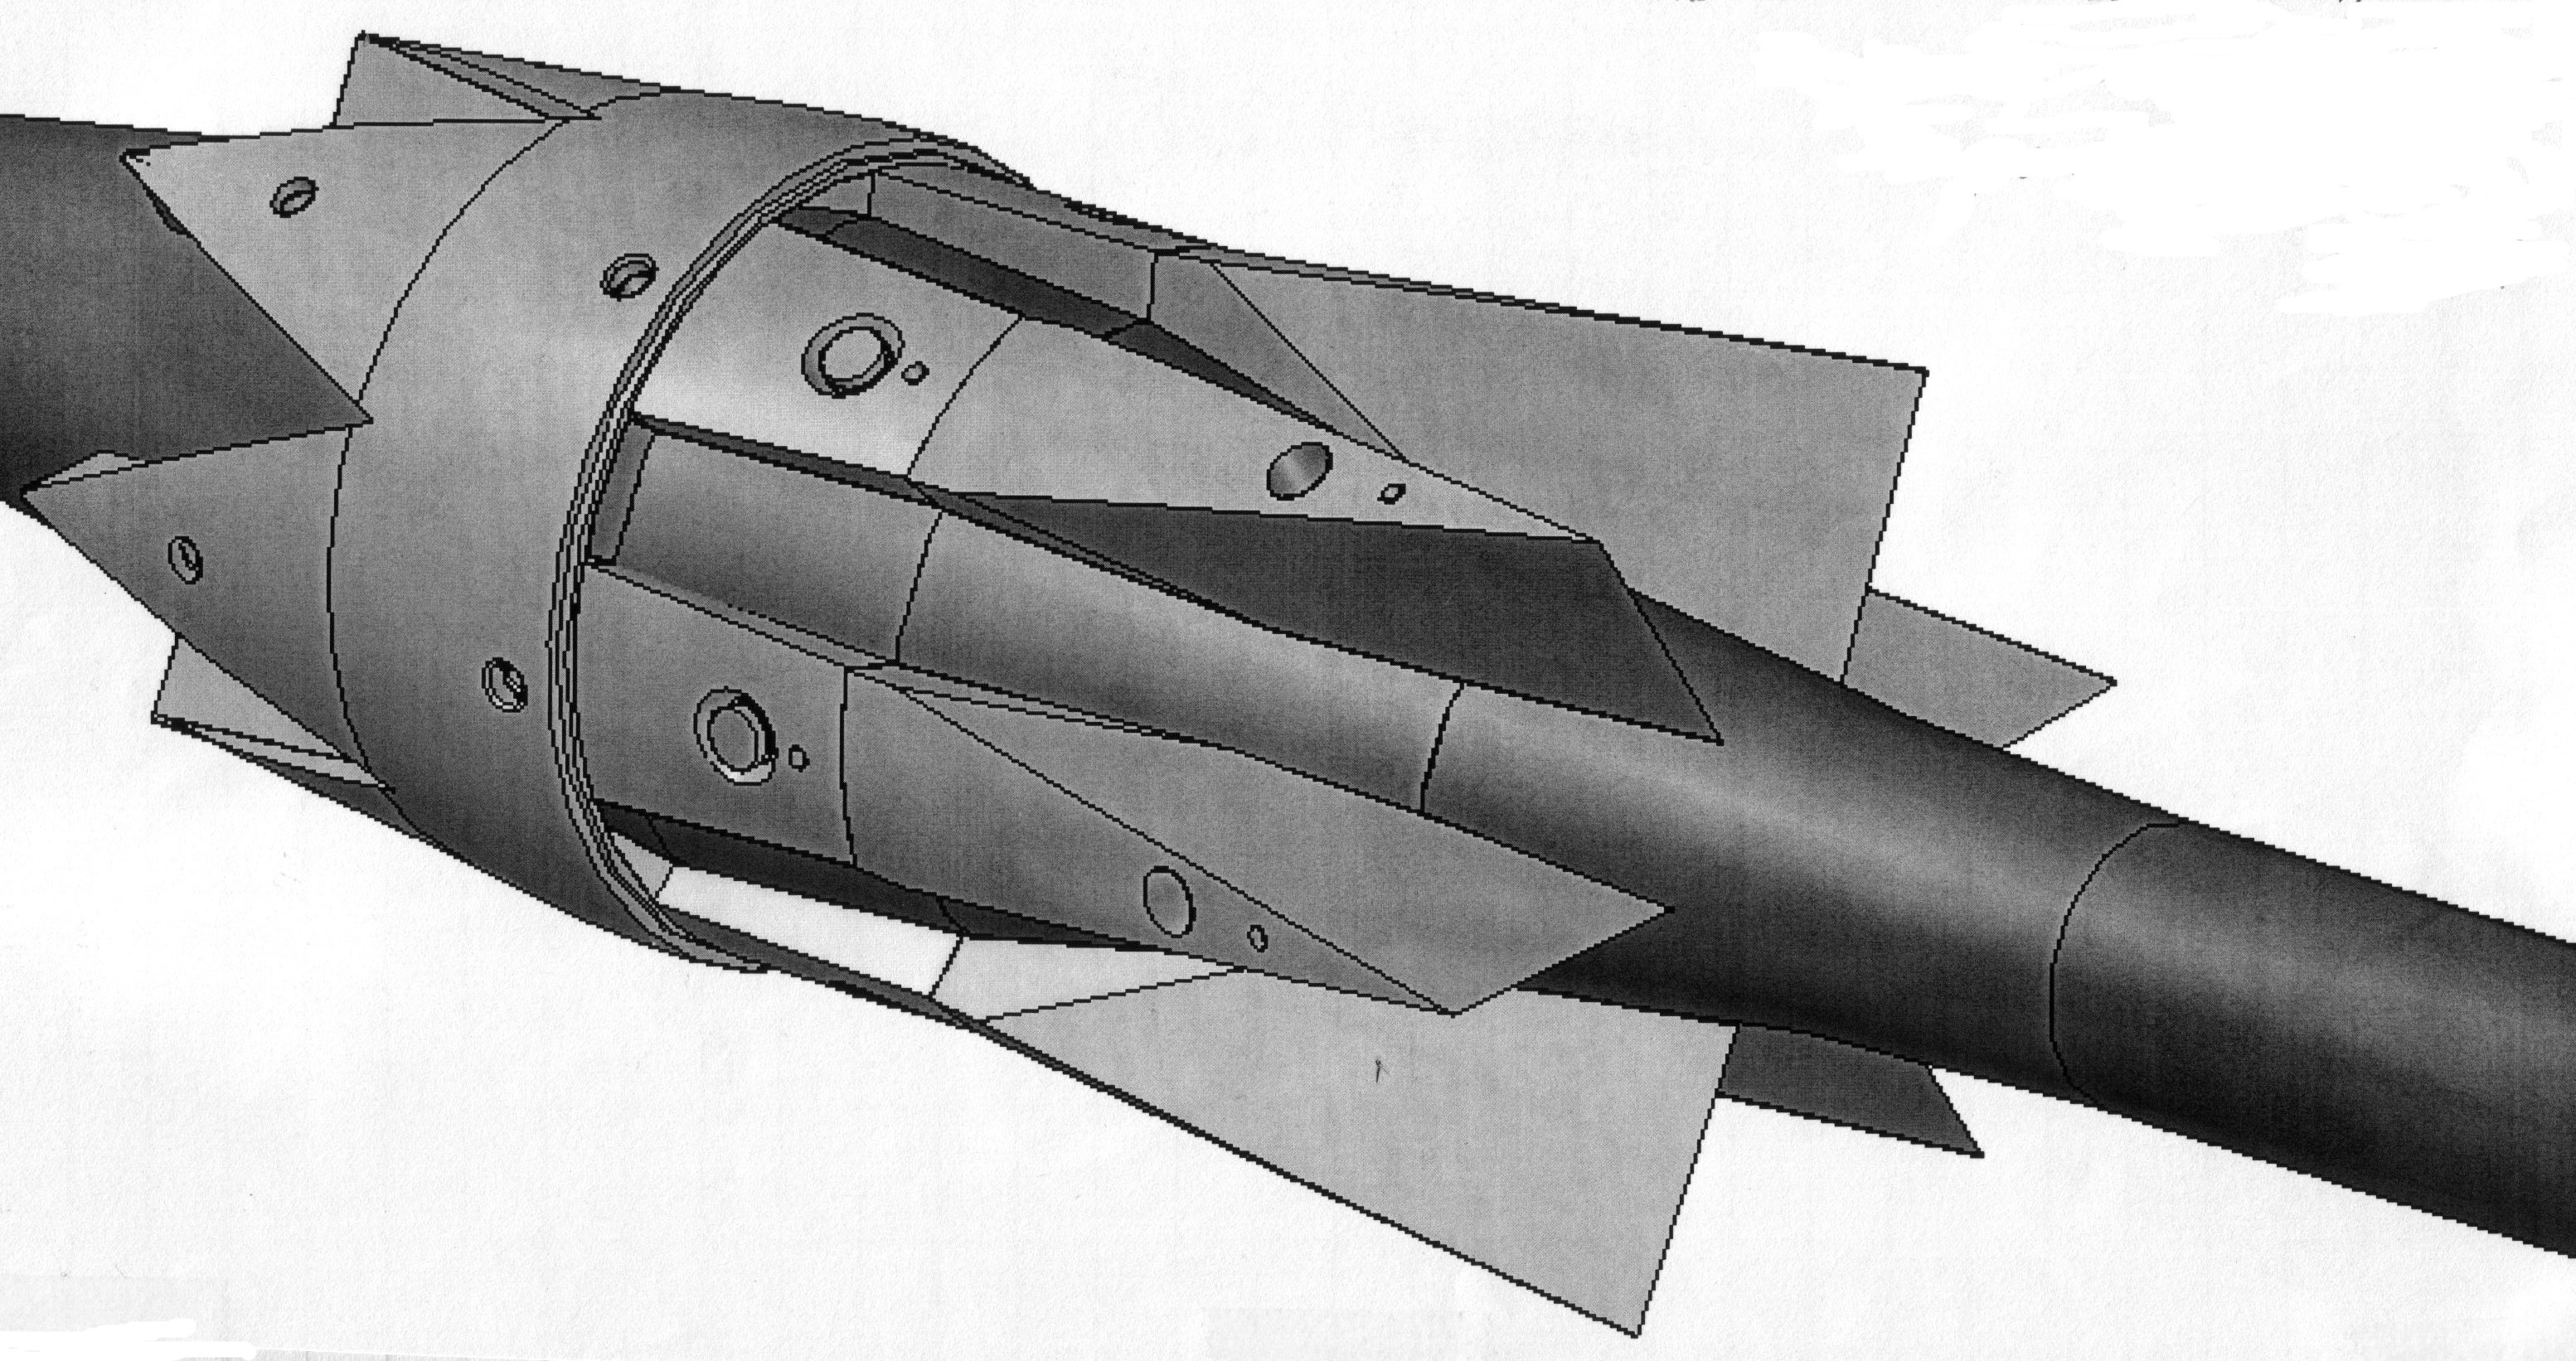
\includegraphics[width=12cm]{../3D/scramjet-1/katsu-scramjet-model.jpg}
\end{center}
\caption{The core section of the scramjet model with the  
  cowl removed from the combustor and nozzle sections 
  to show the individual scramjet ducts between the dividing walls.
  The inlets are at the upper-left of the image.
  This image was scanned from a document provided by Katsu.}
\label{scram1-core-model-fig}
\end{figure}

\begin{figure}[htbp]
\begin{center}
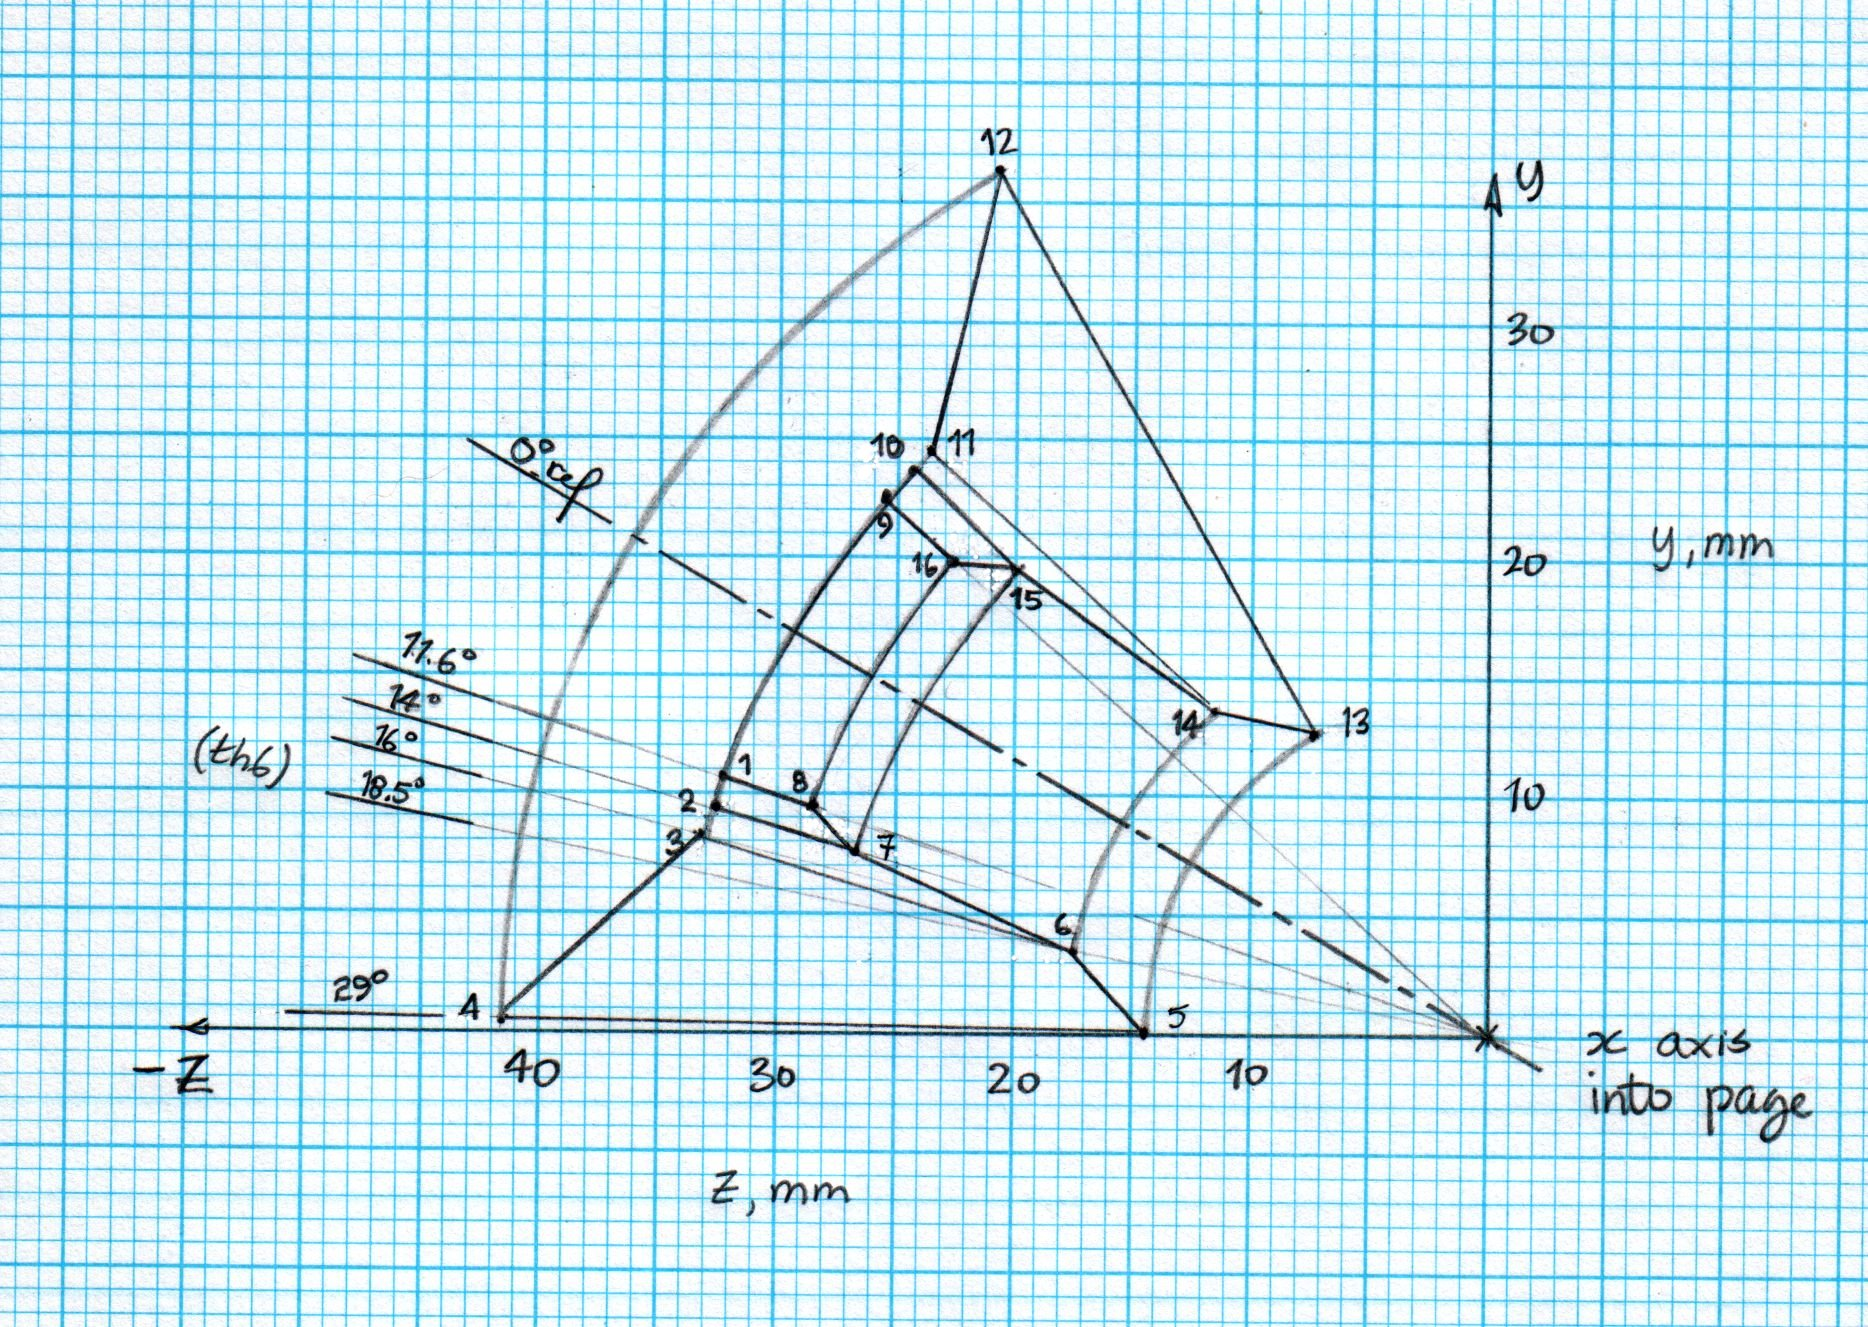
\includegraphics[width=10cm]{../3D/scramjet-1/katsu-scramjet-front-view.jpg}
\end{center}
\caption{Front-view of the wireframe representation of one scramjet duct.
  The labelling of key points corresponds to that used in the job input file
  with the exception that points 9 through 16 were moved to the centre-plane
  of the duct (south surface).}
\label{scram1-front-view-fig}
\end{figure}

\medskip
The geometry for only half of one duct is set up in the job script.
We use a TrianglePatch surface for the side wall (north surface) which is is
somewhat angular; in the original model, it was milled from solid.
The cowl and centre-body surfaces were originally cut on a lathe and so are
curved about the streamwise axis.
These surfaces (top and bottom) are approximated in sections as 
CoonsPatch surfaces and then faceted into TrianglePatch surfaces in order to
join consistently with the side (north and south) walls.
So that the volume is properly closed, the inflow(west) and outflow (east)
surfaces are defined from paths along the edges of the other four surfaces.

\medskip
The simulation is run for only 1000 steps and reaches this point in
a little over 12 minutes on an Intel E2140 @ 1.6GHz (euler).
Compare this with 4 minutes on an LG LS70 laptop computer; we really need to do some
code profiling and optimization.
The presure distribution across some of the surfaces is shown in Figure\,\ref{scram1-p-fig}

\begin{figure}[htbp]
\begin{center}
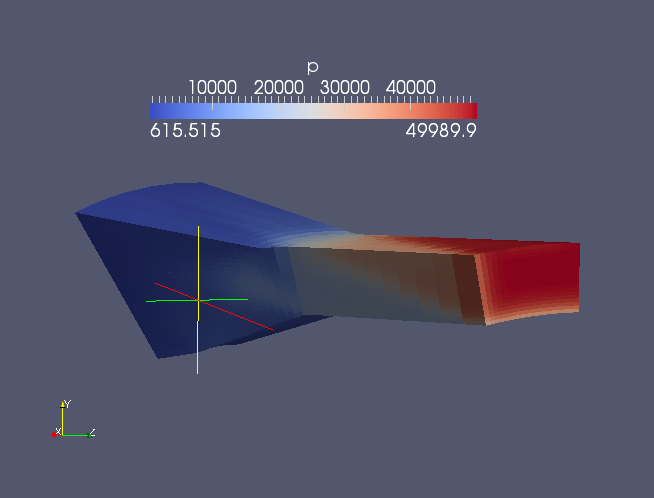
\includegraphics[width=12cm]{../3D/scramjet-1/scram1-p-field.png}
\end{center}
\caption{Pressure distribution on the inlet, combustor, nozzle, and cowl 
  surfaces of the scramjet duct.}
\label{scram1-p-fig}
\end{figure}

\newpage
\subsection{Input script (.py)}
\index{geometric element!PathOnSurface!example of use}
\index{geometric element!CoonsPatch!example of use}
\index{geometric element!TrianglePatch!example of use}
\index{univariate function!LinearFunction!example of use}
\topbar
\lstinputlisting[language={}]{../3D/scramjet-1/scram1.py}
\bottombar
